\subsubsection{Buscar Refacción}
En el siguiente diagrama, la \ref{fig:Diagrama de Secuencia - Eliminar Entrada de Vehículo}, corresponde la secuencia de actividades para buscar algún registro de un empleado en específico, esto para ahorrar un poco más de tiempo en la búsqueda de ducho registro y poder realizar alguna acción sobre ese registro. Existen dos variantes en este proceso:
\begin{itemize}
	\item \textbf{Existe el registro:} Al encontrar el registro en la base de datos, se muestra en pantalla y se podrá interactuar con estos datos.
	\item \textbf{No existe el registro:} Si no se encuentra el registro, se mostrará en pantalla una lista y/o tabla en pantalla.
\end{itemize}
\begin{figure}[!h]
	\centering
	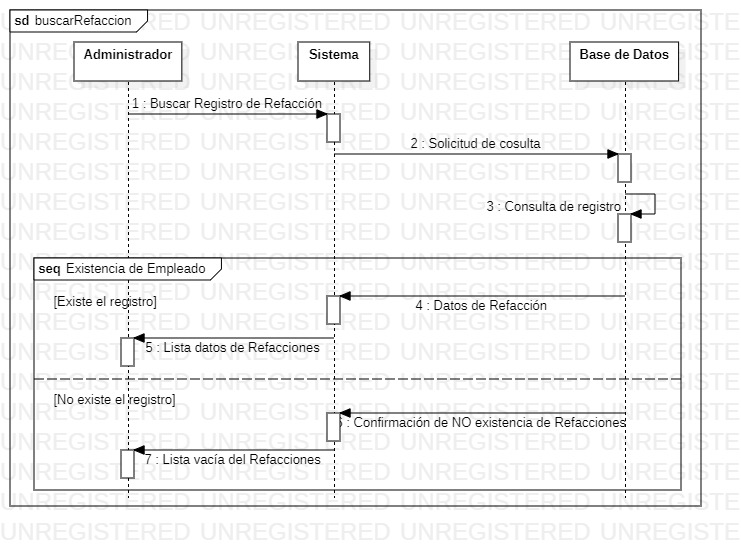
\includegraphics[width=1\textwidth]{./diseno/vprocesos/imagenes/buscarRefaccion}
	\caption{Diagrama de Secuencia - Buscar Refacción}
	\label{fig:Diagrama de Secuencia - Buscar Refaccion}
\end{figure}
\clearpage